
\setsecnumdepth{section}

\chapter{Eigenanalysis}
\label{ch:eigen}

The title of this chapter alone is enough to make one's blood run cold. You
might be thinking, ``even if I could pronounce this, would I want to?''

In German, the root \textit{eigen} (pronounced EYE-gun) means something like
``one's own, inherent thing.'' As we'll see, in studying the eigenvectors and
eigenvalues of a matrix -- which is called eigen-analysis -- we're examining
its deepest, innermost properties. We're peering deep within all the flesh to
see its skeleton. And it turns out this is the key to the most profound
understanding of what a given matrix is and does.

Just look at all the nifty words we'll learn:

\begin{compactitem}
\item \textbf{eigenvector}
\item \textbf{eigenvalue}
\item \textbf{eigendecomposition}
\item \textbf{eigenbasis}
\end{compactitem}

These are all involved in the \textbf{eigenanalysis} of a matrix.

\section{The resonant frequency}

\index{resonant frequency}
\index{frequency, resonant}

We could come at this subject in a bunch of different ways, but let me start
with the first thing that clicked for me when I learned it. At the time, I was
reminded of the phenomenon of a ``resonant frequency'' that some systems
exhibit.

\index{playground}
\index{swing}

You'll remember this effect if you've ever been on a playground swing. When
somebody pushes you (or when you pump your legs to ``push'' yourself) you have
to do it at the right time and at the right pace. The swing has a natural
frequency of oscillation, and it resists being pushed faster or slower than
that. If you find you're swinging from back to front every two seconds, you'll
have to pump your legs every two seconds. Period. Even if you have thighs like
Dwayne Johnson, trying to pump once every 1.5 seconds --  or even furiously at
5 times a second -- will do you no good. Timing it so you pump your legs at
exactly the swing's resonant frequency is the only way to go higher and higher.

\begin{center}
\label{tacoma}
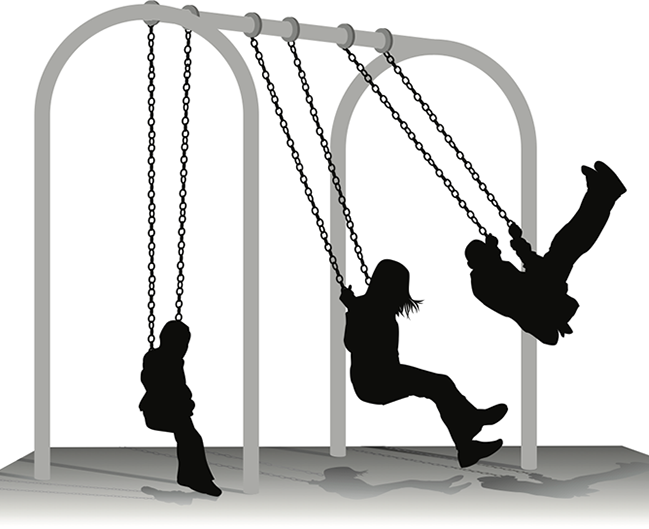
\includegraphics[width=0.45\textwidth]{swing.png}
\quad
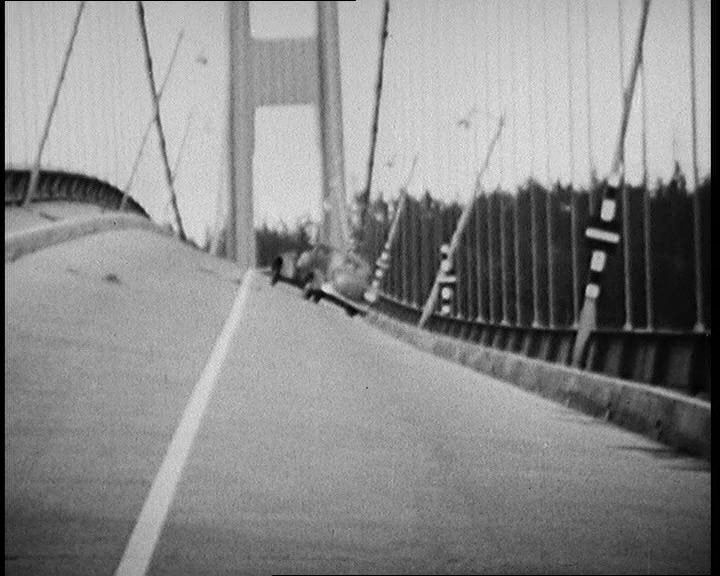
\includegraphics[width=0.45\textwidth]{tacoma.jpg}
\end{center}

\index{Tacoma Narrows Bridge}
\index{bridge}
\index{Slinky}

There are other famous examples of the resonant frequency phenomenon. Perhaps
you've heard of the Tacoma Narrows Bridge (if you've never seen it, check out
the video on
\href{https://www.youtube.com/watch?v=j-zczJXSxnw}{\underline{YouTube}}). It
was a beautiful double-lane suspension bridge in Washington State that crossed
the Puget Sound -- at the time, the third-largest suspension bridge in the
world. Incredibly, on November 7th, 1940, it began to wobble with increasing
intensity as crosswinds dangerously amplified its internal structural
vibrations. It looked like a 3,000-foot-long undulating Slinky.\footnote{The
classic ``Slinky'' toy, by the way, is another example of a system that has a
resonant frequency. You can't make it go down the stairs any faster or slower
than it wants to go.} Moments later, the concrete cracked and split and the
entire bridge completely collapsed and fell into the water. Luckily, drivers
had wisely stopped crossing it minutes before, and the only actual casualty was
a cocker spaniel.

The reasons for the Tacoma Bridge catastrophe are a bit complex, but a key
contributing factor was that a very specific rate of oscillation -- a ``sweet
spot,'' though it was hardly sweet for those involved -- caused the
fluctuations to build on each other instead of being dampened. It's as if the
Tacoma Bridge \textit{wanted} to vibrate at a certain frequency, just like a
playground swing has an intrinsic rhythm that the child can't speed up or slow
down.

\index{guitar}
\index{piano}
\index{middle C}

Yet another example: every non-percussive musical instrument. A piano or guitar
string tuned to middle~C has a certain length and tension, which causes it to
resist vibrations at any frequency other than exactly 262 per second. Thus,
when you strike it, only the 262~Hz\footnote{``Hz,'' pronounced ``hertz,'' is a
unit meaning ``cycles (backs-and-forths) per second.'' Every musical note is
defined by a particular frequency. The lowest key on the piano is 27.5~Hz, and
the highest is 4,186~Hz.} tone gains any traction, and the instrument sounds a
clear, pure note.

\begin{center}
\label{slinky}
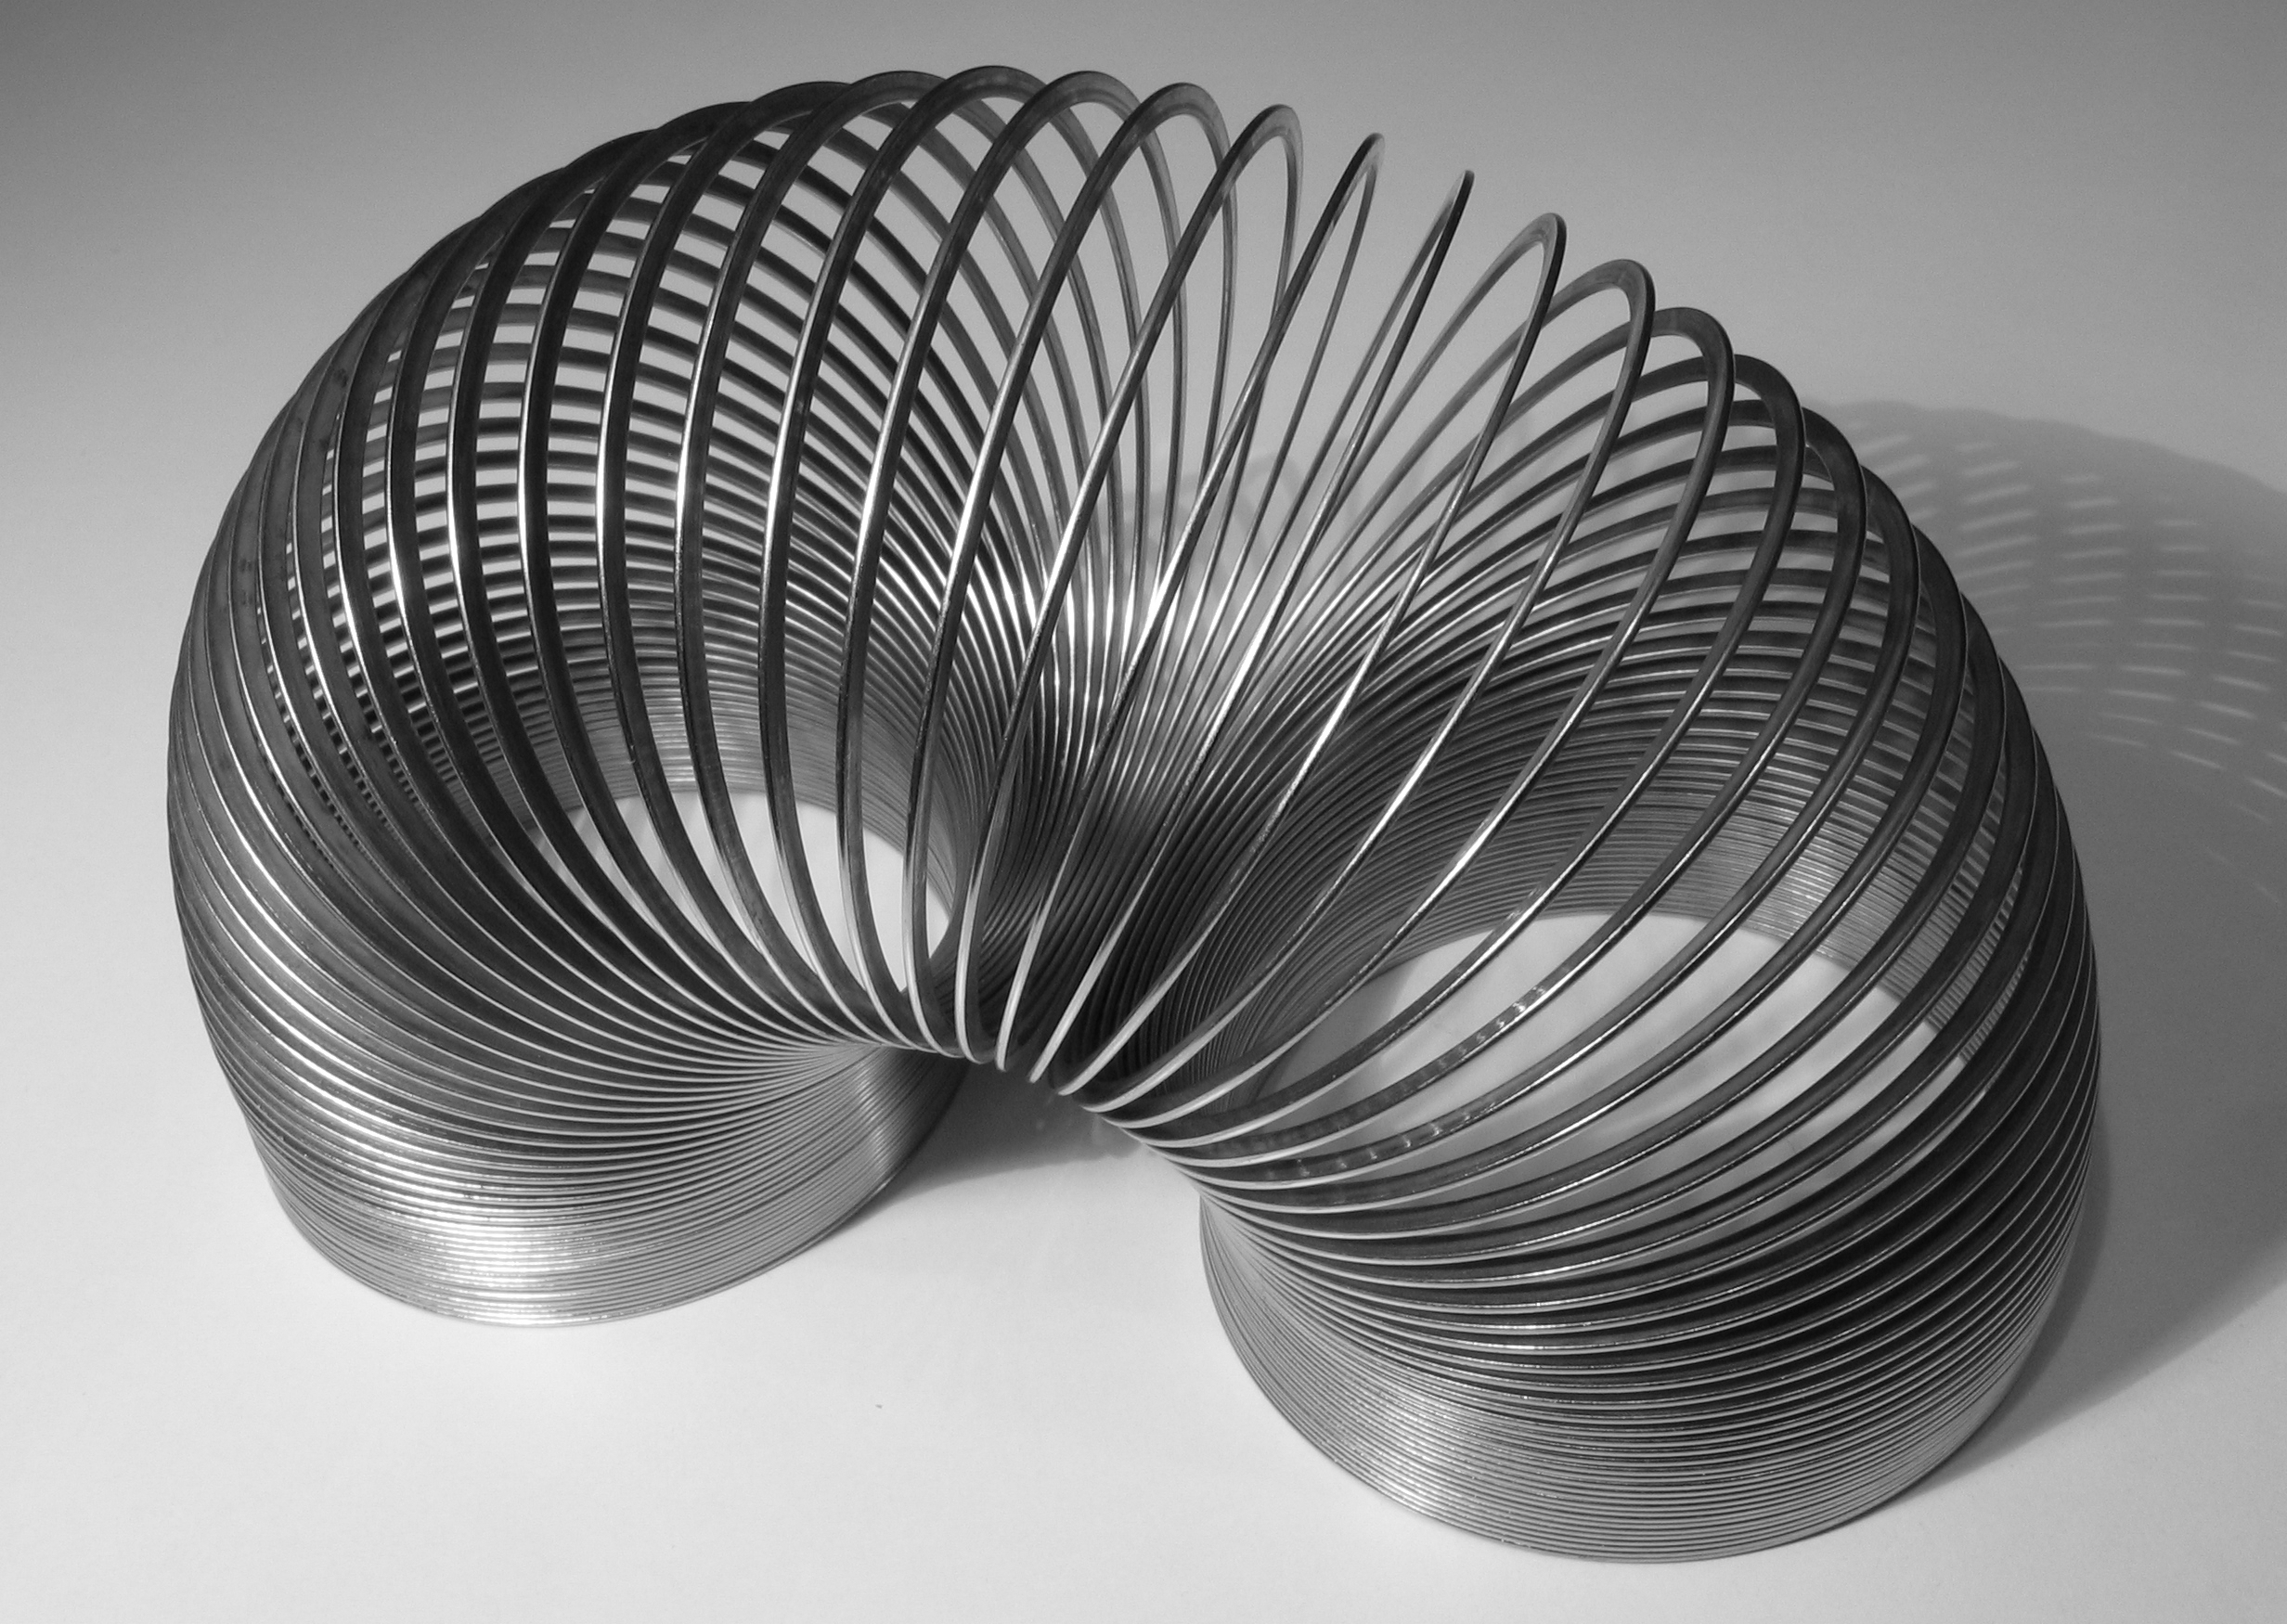
\includegraphics[width=0.45\textwidth]{slinky.jpg}
\quad
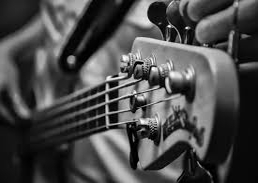
\includegraphics[width=0.45\textwidth]{guitar.jpg}
\end{center}

\section{Linear operators, revisited}

\index{linear operator}

Okay, so what does all this have to do with linear algebra? Well, consider the
linear operators we learned about in Section~\ref{linearOps}
(p.~\pageref{linearOps}). Remember that a linear operator is a square matrix
that transforms one vector into another one of the same dimension when you
left-multiply that vector by the matrix. Let's look at this one:

\begin{align*}
\renewcommand*{\arraystretch}{1.4}
M =
\begin{bmatrix} 
1\frac{1}{2} & -1 \\
\smallskip
-\frac{1}{2} & 1 \\
\end{bmatrix},
\end{align*}

and take it for a spin. If we multiply it by, say, {\footnotesize $\begin{bmatrix} 1
\\ 2 \end{bmatrix}$}, we get:

\begin{align*}
\renewcommand*{\arraystretch}{1.4}
\small
\begin{bmatrix} 
1\frac{1}{2} & -1 \\
\smallskip
-\frac{1}{2} & 1 \\
\end{bmatrix} \cdot
\begin{bmatrix}
1 \\ 2 \\
\end{bmatrix} =
\begin{bmatrix}
-\frac{1}{2} \\ 1\frac{1}{2} \\
\end{bmatrix}, \normalsize \quad \textrm{so}\ 
\boldmath
\begin{bmatrix}
1 \\ 2 \\
\end{bmatrix} \rightarrow \textrm{\textbf{\footnotesize maps to}} \rightarrow
\begin{bmatrix}
-\frac{1}{2} \\ 1\frac{1}{2} \\
\end{bmatrix}.
\unboldmath
\end{align*}

For the input {\footnotesize $\begin{bmatrix} 2 \\ 1 \end{bmatrix}$}, we get:

\vspace{-.2in}
\begin{align*}
\renewcommand*{\arraystretch}{1.4}
\small
\begin{bmatrix} 
1\frac{1}{2} & -1 \\
\smallskip
-\frac{1}{2} & 1 \\
\end{bmatrix} \cdot
\begin{bmatrix}
2 \\ 1 \\
\end{bmatrix} =
\begin{bmatrix}
2 \\ 0 \\
\end{bmatrix}, \normalsize \quad \textrm{so}\ 
\boldmath
\begin{bmatrix}
2 \\ 1 \\
\end{bmatrix} \rightarrow
\begin{bmatrix}
2 \\ 0 \\
\end{bmatrix}.
\unboldmath
\end{align*}

And $M$ maps the input {\footnotesize $\begin{bmatrix} -3 \\ 5 \end{bmatrix}$} to:

\vspace{-.2in}
\begin{align*}
\renewcommand*{\arraystretch}{1.4}
\small
\begin{bmatrix} 
1\frac{1}{2} & -1 \\
\smallskip
-\frac{1}{2} & 1 \\
\end{bmatrix} \cdot
\begin{bmatrix}
-3 \\ 5 \\
\end{bmatrix} =
\begin{bmatrix}
-9\frac{1}{2} \\ 6\frac{1}{2} \\
\end{bmatrix}, \normalsize \quad \textrm{so}\ 
\boldmath
\begin{bmatrix}
-3 \\ 5 \\
\end{bmatrix} \rightarrow
\begin{bmatrix}
-9\frac{1}{2} \\ 6\frac{1}{2} \\
\end{bmatrix}.
\unboldmath
\end{align*}

See a pattern? Me neither. It seems to be all over the place, mapping each
input to some random output with no real rhyme or reason. All of these mappings
are depicted in Figure~\ref{nonEigenvec} (p.~\pageref{nonEigenvec}).

\begin{figure}[ht]
\centering
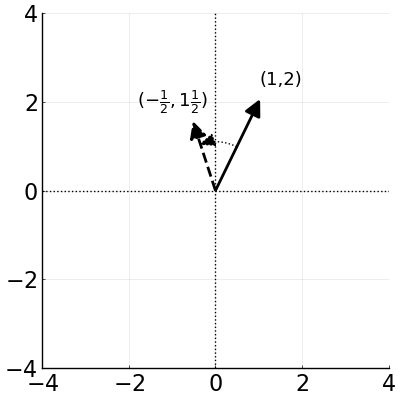
\includegraphics[width=0.4\textwidth]{crazytrans1.png} \quad
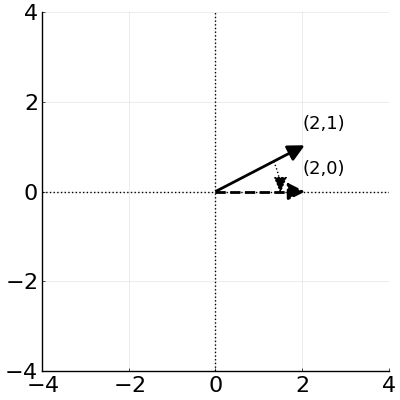
\includegraphics[width=0.4\textwidth]{crazytrans2.png} \\
\smallskip
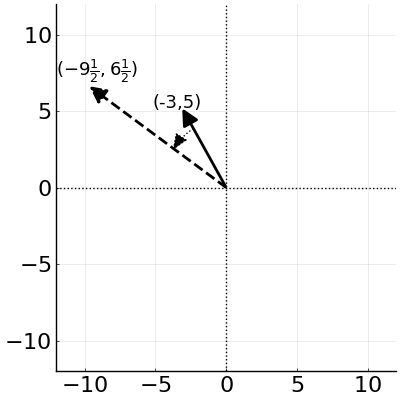
\includegraphics[width=0.4\textwidth]{crazytrans3.png}
\caption{The $M$ matrix's operation. Three randomly-chosen input vectors
(solid) are mapped to crazy output vectors (dashed).}
\label{nonEigenvec}
\end{figure}


\subsection{Hitting a matrix's resonant frequency}

None of that was very special. Random-looking stuff gets mapped to other
random-looking stuff. But now here comes the plot twist. Let's strike this bad
boy at its \textit{resonant frequency}.

% [ 1 1 ], [ -2 1 ]

\vspace{-.2in}
\begin{align*}
\renewcommand*{\arraystretch}{1.4}
\small
\begin{bmatrix} 
1\frac{1}{2} & -1 \\
\smallskip
-\frac{1}{2} & 1 \\
\end{bmatrix} \cdot
\begin{bmatrix}
-1 \\ \frac{1}{2} \\
\end{bmatrix} =
\begin{bmatrix}
-2 \\ 1 \\
\end{bmatrix}, \normalsize \quad \textrm{so}\ 
\boldmath
\begin{bmatrix}
-1 \\ \frac{1}{2} \\
\end{bmatrix} \rightarrow
\begin{bmatrix}
-2 \\ 1 \\
\end{bmatrix}.
\unboldmath
\end{align*}

It's easy to miss the significance of that, so if nothing jumped out at you,
look again. What we just discovered is that the vector {\footnotesize
$\begin{bmatrix} -1 \\ \frac{1}{2} \end{bmatrix}$} is sort of magic: if we feed
it as input to $M$, the output is \textit{a scaled version of the same vector}.
In fact, it exactly doubled in size.

\smallskip

Let's try that again, with the {\footnotesize $\begin{bmatrix} -2 \\ 1
\end{bmatrix}$} we just got back:

\vspace{-.2in}
\begin{align*}
\renewcommand*{\arraystretch}{1.4}
\small
\begin{bmatrix} 
1\frac{1}{2} & -1 \\
\smallskip
-\frac{1}{2} & 1 \\
\end{bmatrix} \cdot
\begin{bmatrix}
-2 \\ 1 \\
\end{bmatrix} =
\begin{bmatrix}
-4 \\ 2 \\
\end{bmatrix}, \normalsize \quad \textrm{so}\ 
\boldmath
\begin{bmatrix}
-2 \\ 1 \\
\end{bmatrix} \rightarrow
\begin{bmatrix}
-4 \\ 2 \\
\end{bmatrix}.
\unboldmath
\end{align*}

Boom. It exactly doubled again. And if we then feed it {\footnotesize
$\begin{bmatrix} -4 \\ 2 \end{bmatrix}$}:

\vspace{-.2in}
\begin{align*}
\renewcommand*{\arraystretch}{1.4}
\small
\begin{bmatrix} 
1\frac{1}{2} & -1 \\
\smallskip
-\frac{1}{2} & 1 \\
\end{bmatrix} \cdot
\begin{bmatrix}
-4 \\ 2 \\
\end{bmatrix} =
\begin{bmatrix}
-8 \\ 4 \\
\end{bmatrix}, \normalsize \quad \textrm{so}\ 
\boldmath
\begin{bmatrix}
-4 \\ 2 \\
\end{bmatrix} \rightarrow
\begin{bmatrix}
-8 \\ 4 \\
\end{bmatrix}.
\unboldmath
\end{align*}

\index{piano}
\index{middle C}

Boom. It exactly doubled again. This is very intriguing. Vectors in this one
particular direction aren't ``jumping around'' like the other ones did when $M$
acted on them. Instead, the matrix just plays them back for us (at twice the
volume) like a pure middle C singing out from a piano. Figure~\ref{eigenvec1}
(p.~\pageref{eigenvec1}) shows the illustration.

\begin{figure}[ht]
\centering
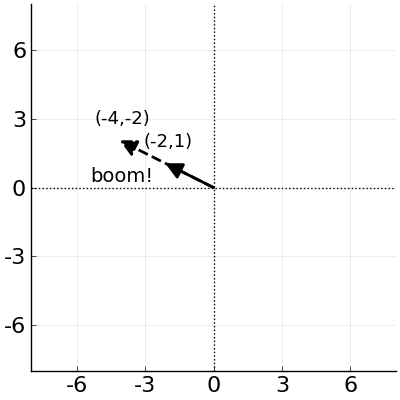
\includegraphics[width=0.4\textwidth]{eigentrans1.png} \quad
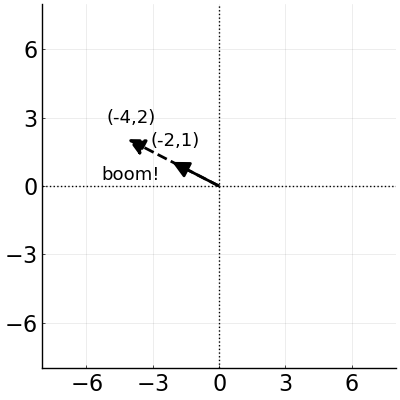
\includegraphics[width=0.4\textwidth]{eigentrans2.png} \\
\smallskip
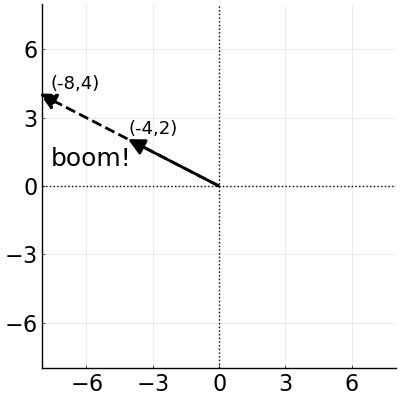
\includegraphics[width=0.4\textwidth]{eigentrans3.png}
\caption{The $M$ matrix's operation when applied to one of its eigenvectors.
The input (solid) is mapped to the \textit{same} vector, but scaled (dashed).}
\label{eigenvec1}
\end{figure}

\pagebreak
\index{eigenvector}
\index{eigenvalue}

Big concept: the vector {\footnotesize $\begin{bmatrix} -1 \\ \frac{1}{2}
\end{bmatrix}$} (and all its multiples, like {\footnotesize $\begin{bmatrix} -2
\\ 1 \end{bmatrix}$}, {\footnotesize $\begin{bmatrix} -4 \\ 2 \end{bmatrix}$},
$\dots$) is called an \textbf{eigenvector} of $M$. Here's what that means:

\begin{framed}
An \textbf{eigenvector} of a matrix $A$ is any vector that gets mapped to a
scaled version of \textit{itself} -- \textit{i.e.}, to a vector in the same
direction -- when muliplied by $A$. In symbols, for an eigenvector
$\overrightarrow{\textbf{x}}$:

{\centering
$ \displaystyle
A \overrightarrow{\textbf{x}} = \lambda \overrightarrow{\textbf{x}}$ \\
}

for some number $\lambda$. And that number $\lambda$ is called an
\textbf{eigenvalue} of $A$.
\end{framed}

In this case, the eigenvalue $\lambda$ is 2, since any vector in the
{\footnotesize $\begin{bmatrix} -1 \\ \frac{1}{2} \end{bmatrix}$} direction
gets multiplied by 2.

\subsection{Alternate resonant frequencies}

Just curious, are there any \textit{other} ``magic'' vectors for our $M$
matrix? It turns out there are. Try {\footnotesize $\begin{bmatrix} 4 \\ 4
\end{bmatrix}$}:

\vspace{-.2in}
\begin{align*}
\renewcommand*{\arraystretch}{1.4}
\small
\begin{bmatrix} 
1\frac{1}{2} & -1 \\
\smallskip
-\frac{1}{2} & 1 \\
\end{bmatrix} \cdot
\begin{bmatrix}
4 \\ 4 \\
\end{bmatrix} =
\begin{bmatrix}
2 \\ 2 \\
\end{bmatrix}, \normalsize \quad \textrm{so}\ 
\boldmath
\begin{bmatrix}
4 \\ 4 \\
\end{bmatrix} \rightarrow
\begin{bmatrix}
2 \\ 2 \\
\end{bmatrix}.
\unboldmath
\end{align*}

So giving {\footnotesize $\begin{bmatrix} 4 \\ 4 \end{bmatrix}$} to the $M$
linear operator produces a \textit{shrunken} version of the input: exactly half
as long. And of course this pattern repeats for any vector in the
{\footnotesize $\begin{bmatrix} 4 \\ 4 \end{bmatrix}$} direction:

\vspace{-.2in}
\begin{align*}
\renewcommand*{\arraystretch}{1.4}
\small
\begin{bmatrix} 
1\frac{1}{2} & -1 \\
\smallskip
-\frac{1}{2} & 1 \\
\end{bmatrix} \cdot
\begin{bmatrix}
2 \\ 2 \\
\end{bmatrix} =
\begin{bmatrix}
1 \\ 1 \\
\end{bmatrix}, \normalsize \quad \textrm{so}\ 
\boldmath
\begin{bmatrix}
2 \\ 2 \\
\end{bmatrix} \rightarrow
\begin{bmatrix}
1 \\ 1 \\
\end{bmatrix},
\unboldmath
\end{align*}

and so forth. This means that {\footnotesize $\begin{bmatrix} 4 \\ 4
\end{bmatrix}$} (and every other vector in the same direction) is also an
eigenvector of $M$, this time with eigenvalue $\lambda=\frac{1}{2}$.

\bigskip

Wow, okay. And does $M$ have still other eigenvectors in store for us as well?
The answer turns out to be \textbf{\textit{no,}} an important fact we'll return
to in a moment.

\medskip

\index{dominant eigenvector}

To recap, then, our matrix $M$ has two eigenvectors: {\scriptsize
$\begin{bmatrix} -1 \\ \frac{1}{2} \end{bmatrix}$} (and any multiple of it) and
{\scriptsize $\begin{bmatrix} 4 \\ 4 \end{bmatrix}$} (and any multiple of it).
The first of these has eigenvalue 2, and the second has eigenvalue
$\frac{1}{2}$. Also, we have a special name for the {\scriptsize
$\begin{bmatrix} -1 \\ \frac{1}{2} \end{bmatrix}$} vector: it's called the
\textbf{dominant eigenvector}, for reasons you'll see in a moment. A matrix's
dominant eigenvector is simply the eigenvector with the highest eigenvalue.

\section{Magnetic pull}

Now if you followed all that, \textit{this} is sure to absolutely blow your
mind. I know it did mine. I'm going to feed a random vector in as an input to
our $M$ matrix, and then repeatedly put its output back in to $M$ and see where
it goes. Remember that if I do this with an \textit{eigenvector}, I'll keep
getting back progressively scaled copies of the input vector. But let's see
what happens when we pass in an ordinary, non-special, non-eigen vector.

I'll choose {\footnotesize $\begin{bmatrix} 1 \\ 2\frac{1}{2} \end{bmatrix}$}
just for giggles, and call it $\overrightarrow{\textbf{r}}$ for ``random.'' If
I keep multiplying $\overrightarrow{\textbf{r}}$ by $M$, here's what I get:

\vspace{-.2in}
\begin{align*}
\renewcommand*{\arraystretch}{1.4}
\small
\overrightarrow{\textbf{r}} &=
\boldmath
\begin{bmatrix}
1 \\ 2\frac{1}{2} \\
\end{bmatrix}, \quad \textrm{ \ding{182}} \\
\unboldmath
\begin{bmatrix} 
1\frac{1}{2} & -1 \\
\smallskip
-\frac{1}{2} & 1 \\
\end{bmatrix} \cdot
\begin{bmatrix}
1 \\ 2\frac{1}{2} \\
\end{bmatrix} &=
\boldmath
\begin{bmatrix}
-1 \\ 2 \\
\end{bmatrix}, \quad \textrm{ \ding{183}} \\
\unboldmath
\begin{bmatrix} 
1\frac{1}{2} & -1 \\
\smallskip
-\frac{1}{2} & 1 \\
\end{bmatrix} \cdot
\begin{bmatrix}
-1 \\ 2 \\
\end{bmatrix} &=
\boldmath
\begin{bmatrix}
-3\frac{1}{2} \\ 2\frac{1}{2} \\
\end{bmatrix}, \quad \textrm{ \ding{184}} \\
\unboldmath
\begin{bmatrix} 
1\frac{1}{2} & -1 \\
\smallskip
-\frac{1}{2} & 1 \\
\end{bmatrix} \cdot
\begin{bmatrix}
-3\frac{1}{2} \\ 2\frac{1}{2} \\
\end{bmatrix} &=
\boldmath
\begin{bmatrix}
-7\frac{3}{4} \\ 4\frac{1}{4} \\
\end{bmatrix}... \quad \textrm{ \ding{185}} \\
\unboldmath
\end{align*}

You might say ``big deal'' until you look at the upper left of
Figure~\ref{converge1}, where I've plotted this sequence of vectors with the
circled numbers \ding{182}, \ding{183}, \ding{184}, and \ding{185}. I've also
plotted \textit{the dominant eigenvector as a dotted line} on this plot. Look
at what happens: every time we multiply by $M$, that random old vector is
pulled towards $M$'s dominant eigenvector (which was in the direction
{\footnotesize $\begin{bmatrix} -1 \\ \frac{1}{2} \end{bmatrix}$}, as you
recall) like a magnet! And incredibly, this happens with \textit{any} vector I
start with. The other panes of Figure~\ref{converge1} shows what happens when I
start with {\footnotesize $\begin{bmatrix} -2 \\ -1 \end{bmatrix}$},
{\footnotesize $\begin{bmatrix} -1 \\ -2 \end{bmatrix}$},
and {\footnotesize $\begin{bmatrix} 2 \\ \frac{1}{2} \end{bmatrix}$}. Resonant
frequency indeed!

\begin{figure}[ht]
\centering
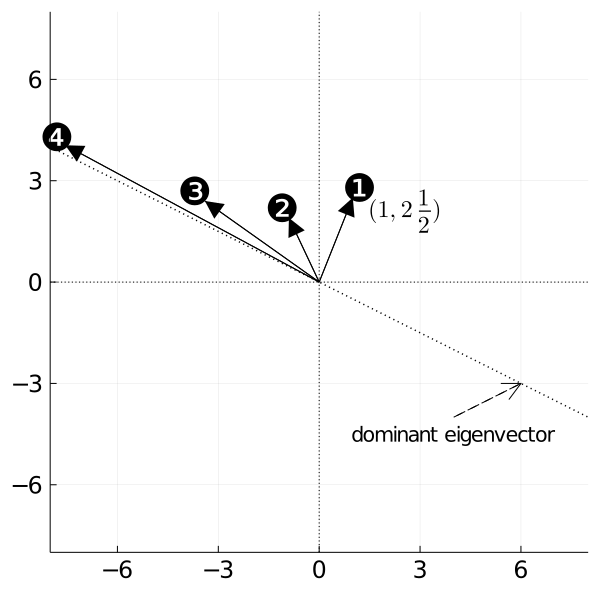
\includegraphics[width=0.4\textwidth]{converge1.png} \quad
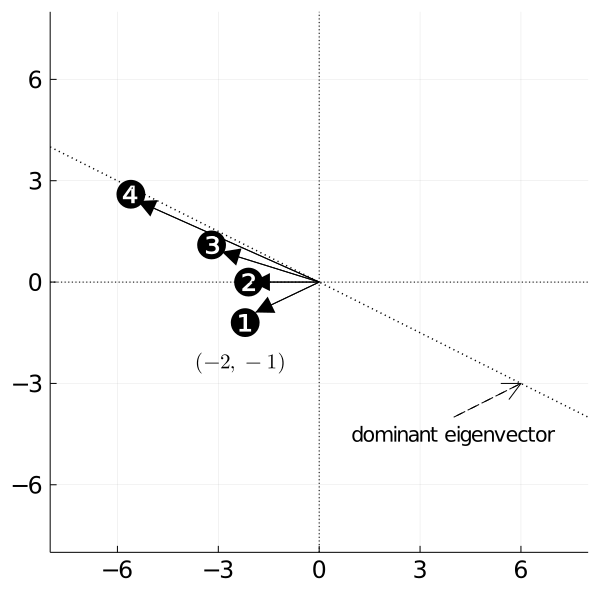
\includegraphics[width=0.4\textwidth]{converge2.png} \\
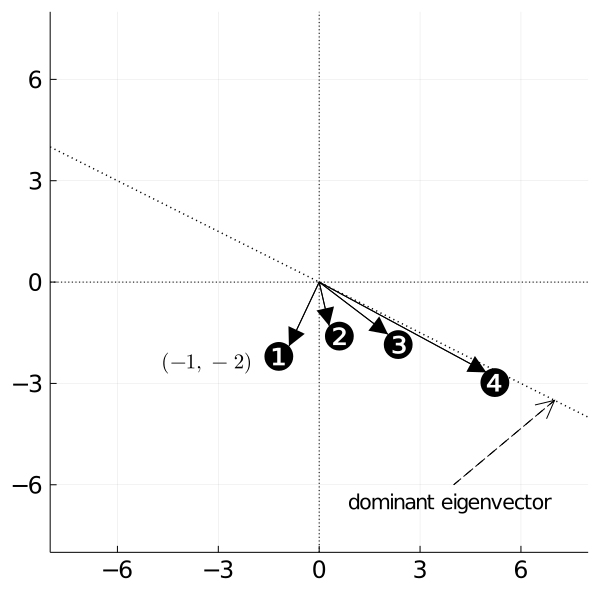
\includegraphics[width=0.4\textwidth]{converge3.png} \quad
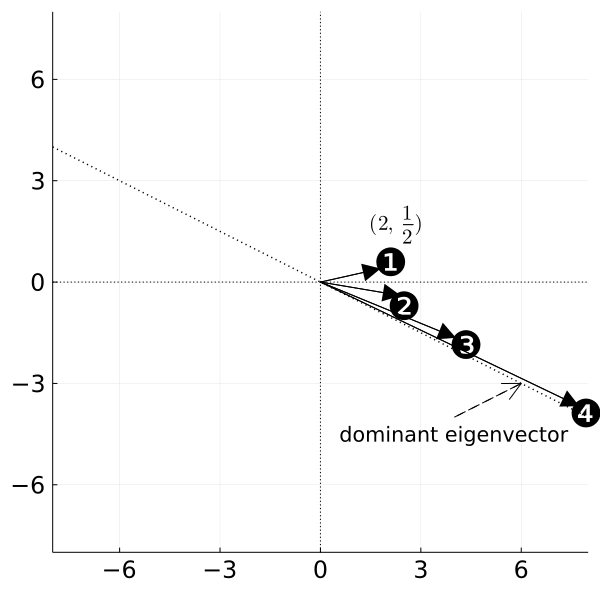
\includegraphics[width=0.4\textwidth]{converge4.png}
\caption{Holy cow -- repeatedly applying the $M$ operator by any vector at all
drags it progressively to the dominant eigenvector!}
\label{converge1}
\end{figure}

So we see that the dominant eigenvector is dominant indeed. The matrix somehow
\textit{wants} to map its inputs to the direction of the dominant eigenvector,
and if you keep pushing its button, it'll always be drawn there. And that's
true \textit{no matter where you started.} This fact will have immense
repercussions when we look at things like Markov chains and the PageRank
algorithm in the next chapter.

In fact, the only vector I can start with and not get dragged to the dominant
eigenvector is one that is \textit{exactly} in the direction of the
\textit{other} eigenvector. As noted previously, if we give $M$ the input
{\footnotesize $\begin{bmatrix} 4 \\ 4 \end{bmatrix}$} (or anything in that
direction), it will stay locked in that direction (a 45\textdegree~angle
counterclockwise from the x-axis) and shrink by half each time. But if we nudge
that vector even slightly away from that other eigenvector -- say,
{\footnotesize $\begin{bmatrix} 4 \\ 4.0001 \end{bmatrix}$} -- it'll get pulled
to the dominant eigenvector's direction ({\footnotesize $\begin{bmatrix} -1 \\
\frac{1}{2} \end{bmatrix}$}) instead.

\bigskip

In terms of our previous analogy, we're witnessing an even stronger sort of
``resonant frequency.'' With a playground swing, if we pump our legs at the
wrong pace, nothing much happens -- the swing just deadens. But imagine if
pumping our legs at the wrong pace got automatically \textit{converted} to the
right pace? In real life, if an operatic soprano sings just the right piercing
note, she can shatter a nearby glass. But what if no matter what note she sang,
it was automatically adjusted by the glass to \textit{be} just the perfect tone
to shatter the glass? What we have here is not only a resonant frequency, but a
magnet pulling every vector \textit{towards} the resonant frequency. Amazing.

% change of basis

% eigenbasis: the natural basis

% decomposition

% spectral theorem

